\documentclass[conference]{IEEEtran}
\IEEEoverridecommandlockouts
\usepackage{cite}
\usepackage{amsmath,amssymb}
\usepackage{graphicx}
\usepackage{booktabs}
\usepackage{array}
\usepackage{tabularx}
\usepackage{url}
\usepackage{xcolor}
\usepackage{algorithm}
\usepackage{algpseudocode}
\usepackage{tikz}
\usetikzlibrary{positioning,arrows.meta,fit,backgrounds}

% Includes an image if it exists, otherwise a framed placeholder (so the file always compiles).
\newcommand{\img}[2]{%
  \IfFileExists{figures/#1}{\includegraphics[width=#2]{figures/#1}}{%
  \fbox{\parbox{\dimexpr#2-2\fboxsep-2\fboxrule\relax}{\centering\vspace{1.5em}\textcolor{red}{missing figures/#1}\vspace{1.5em}}}}}

\begin{document}

\title{EdgePark: Real-Time Restricted-Zone Parking Violation Detection with Tracking and Dwell Time on a Simulated Raspberry Pi~5 Edge Node}

\author{
\IEEEauthorblockN{Abdullah Attique (23i-0073)}
\IEEEauthorblockA{Department of Artificial Intelligence\\
FAST-NUCES, Islamabad, Pakistan\\
abdullah.attique.2005@gmail.com}
\and
\IEEEauthorblockN{Minahil Rizwan (23i-0114)}
\IEEEauthorblockA{Department of Artificial Intelligence\\
FAST-NUCES, Islamabad, Pakistan\\
minahil.rizwan99@gmail.com}
\and
\IEEEauthorblockN{Talha Akram (\textcolor{red}{23i-XXXX})}
\IEEEauthorblockA{Department of Artificial Intelligence\\
FAST-NUCES, Islamabad, Pakistan\\
\textcolor{red}{email}}
}

\maketitle

\begin{abstract}
Vehicles left in fire lanes, entrances and no-parking curbs block access and safety routes, yet most camera-based violation detectors judge every video frame on its own and run on servers or GPUs. We present EdgePark, an edge system that detects parking violations next to the camera and sends only short alerts. A COCO-pretrained YOLO26n detector exported to ONNX finds vehicles, ByteTrack keeps their identities, and a dwell-time rule raises one alert only after a vehicle has stood still inside a restricted zone for $T$ seconds. Alerts with a privacy-filtered snapshot travel over MQTT to a live web dashboard. Because no Raspberry Pi was available, the edge node runs in a Docker container whose CPU limit is calibrated to the published Raspberry Pi~5 speed (302 ms vs.\ 299 ms per image). We compare three nano detectors on 842 UA-DETRAC frames, three runtime formats on the simulated Pi~5, and the alert logic on 16 public parking-violation videos with a development/test split. YOLO26n is the most accurate model (mAP@0.5:0.95 = 0.582) and ONNX makes it 35\% faster (187 ms). On the eleven test videos a frame-wise region-of-interest baseline produces 1,776 alerts for 9 violations (precision 0.005); EdgePark produces 9 alerts, all correct, at $T = 30$ s (precision 1.000, recall 0.900) and 5 correct alerts at $T = 60$ s. The full system runs at about 4 frames per second at Pi~5 speed, and alerts reach the dashboard 0.3--0.9 s after the frame is captured. The calibration holds for the PyTorch runtime but not for ONNX and NCNN, so runtime rankings from an x86 simulation should not be carried over to ARM boards.
\end{abstract}

\begin{IEEEkeywords}
edge computing, parking violation detection, YOLO, multi-object tracking, dwell time, MQTT, Raspberry Pi
\end{IEEEkeywords}

%=====================================================================
\section{Introduction}
%=====================================================================
Illegal parking in places that must stay free is a daily problem on campuses and in small towns. A car standing in a fire lane, in front of a gate or along a no-parking curb blocks emergency vehicles and other traffic. Patrols cannot watch every spot all the time, and streaming every CCTV camera to a central server costs bandwidth, storage and a reliable network, and moves images of people and number plates off site.

Edge computing offers another option: a small computer next to the camera analyses the video and sends only the result. Nano versions of the YOLO detector family are small enough for boards such as the Raspberry Pi. Da Luz et al.~\cite{daluz2026} recently counted vehicles in a parking lot with YOLOv8--v11 and a pixel-wise region of interest (ROI), and measured 1 to 92 s per image on a Raspberry Pi~3 and~4. Their work, like most violation detectors, decides frame by frame whether a vehicle box lies in the region. Such a rule cannot tell a parked car from a car driving through, and it reports the same parked car again in every frame.

This project builds and evaluates a complete edge pipeline that turns detections into violation \emph{events}. Our research questions are:
\begin{itemize}
\item \textbf{RQ1:} How do recent nano YOLO models and optimised runtimes compare in accuracy and speed on a Raspberry Pi~5 class device?
\item \textbf{RQ2:} How much do tracking and a dwell-time rule reduce false and duplicate alerts compared with frame-wise ROI detection?
\item \textbf{RQ3:} Which model and runtime give the best balance for deployment, and how well does a CPU-limited container stand in for a real board?
\end{itemize}

The contributions are:
\begin{enumerate}
\item An end-to-end edge system: RTSP camera stream, detector, ByteTrack tracking, polygon zones, stationary-aware dwell timer, duplicate merging, privacy blurring, MQTT alerts with heartbeat and last-will, and a live dashboard, all deployed with Docker.
\item A Raspberry Pi~5 simulation: a container whose CPU limit is calibrated to a published Pi~5 benchmark, and a test of whether that calibration transfers to other runtimes.
\item An evaluation of three nano detectors (YOLOv8n, YOLO11n, YOLO26n) on 842 UA-DETRAC frames and in three formats (PyTorch, ONNX, NCNN) on the simulated Pi~5.
\item An alert-level evaluation on 16 public videos with a written zone policy, a dev/test split, a replicated frame-wise baseline, an ablation of every component and a threshold study.
\item A public, reproducible repository with code, zones, ground truth and result files.
\end{enumerate}

%=====================================================================
\section{Related Work}
%=====================================================================
\textit{Region-based violation detectors.} Most systems combine a detector with a hand-drawn region. Makmur et al.~\cite{makmur2025} flag a motorcycle when at least half of its YOLOv7 box overlaps a no-parking region (F1 86.2\%), and Bakri et al.~\cite{bakri2026} add YOLOv12 segmentation and vehicle orientation (F1 92.68\%). Peng et al.~\cite{peng2022} detect six illegal-parking situations from a camera on a moving car with YOLOv3 at 0.07 s per image on a GPU. These systems test one model and give each frame its own verdict.

\textit{Time rules and tracking.} Gao et al.~\cite{gao2022} call a vehicle illegally parked when it stays in a curb lane for more than 10 s and reach a precision of 85.8\% at their best site. Sharma et al.~\cite{sharma2023} track campus vehicles with YOLOv8x and DeepSORT or OC-SORT and check how long each identity stays. Cahyono et al.~\cite{cahyono2026} show that ByteTrack~\cite{zhang2022bytetrack} identities stop a vehicle from being counted twice. None of these works measures how many false or duplicate alerts the time rule and the tracker remove compared with a frame-wise rule.

\textit{Model choice and edge speed.} Surveys of the YOLO family~\cite{sapkota2025} and benchmarks in driving assistance~\cite{chaman2026} and on an embedded robot car~\cite{reveles2025} show that newer versions are usually, but not always, more accurate. Parking studies compare YOLOv5, v7-tiny and v8~\cite{garta2025} or add attention blocks~\cite{zhao2024}, mostly with GPU timings. Kim et al.~\cite{kim2025} report 227 ms per image for YOLOv8n on an embedded box, and a recent review~\cite{yunganina2026} finds that 8 of 15 parking studies give no speed figures at all. The base paper~\cite{daluz2026} ran plain PyTorch on Pi~3 and Pi~4 and named model conversion and the Pi~5 as future work.

\textit{Gap.} Table~\ref{tab:related} summarises the studies. No previous work combines (i) a comparison of current nano models and runtimes on a Pi~5 class device, (ii) an alert-level comparison of frame-wise and dwell-time logic on the same videos, and (iii) a complete deployable pipeline with messaging and a dashboard. When no board is available, a CPU-limited container is a common stand-in, but its validity across runtimes has not been checked.

\begin{table*}[!t]
\caption{Related work by system component (\checkmark{} = present, -- = absent)}
\label{tab:related}
\centering
\footnotesize
\setlength{\tabcolsep}{4pt}
\begin{tabularx}{\textwidth}{@{}p{2.3cm}p{2.6cm}p{2.2cm}cccp{2.4cm}X@{}}
\toprule
Study & Detector & Zone test & Tracking & Time rule & Edge device & Reported result & Missing for our goal \\
\midrule
da Luz \cite{daluz2026} & YOLOv8--v11 (n, x) & Box centre in mask & -- & -- & Pi 3 / Pi 4 & Bal. acc. 99.68\%; 1--92 s/image & Frame-wise; no alerts; plain PyTorch \\
Makmur \cite{makmur2025} & YOLOv7 & Box overlap $\geq$50\% & -- & -- & -- & F1 86.2\% & One model; frame-wise \\
Bakri \cite{bakri2026} & YOLOv12-seg & Mask + orientation & -- & -- & -- & F1 92.68\% & No speed; frame-wise \\
Peng \cite{peng2022} & YOLOv3 & Scene rules & -- & -- & GPU & F 90.66\%; 0.07 s & Moving camera; no edge board \\
Gao \cite{gao2022} & YOLOv3 & Lane filter & -- & \checkmark{} (10 s) & -- & P 85.8\% & Effect of time rule not isolated \\
Sharma \cite{sharma2023} & YOLOv8x & Parking area & \checkmark{} & \checkmark{} & GPU & MOTA 0.90--1.00 & No comparison with frame-wise alerts \\
Cahyono \cite{cahyono2026} & YOLOv8s & Counting line & \checkmark{} & -- & -- & F1 0.930 & Counting, not parking \\
Kim \cite{kim2025} & YOLOv8n & Parking slots & -- & voting & Embedded box & 227 ms/image & Occupancy, not violations \\
\midrule
\textbf{EdgePark (ours)} & YOLOv8n / 11n / 26n; PT, ONNX, NCNN & Ground point in polygon & \checkmark{} & \checkmark{} & Pi 5 (calibrated container) & P 1.000, R 0.900 (test, 30 s); 187 ms/image & -- \\
\bottomrule
\end{tabularx}
\end{table*}

%=====================================================================
\section{System Design and Implementation}
%=====================================================================
\subsection{Architecture}
Fig.~\ref{fig:arch} shows the system. It consists of four services that run as Docker containers on one host and communicate only over the network, as separate devices would:
\begin{itemize}
\item \textbf{Camera:} a MediaMTX server with ffmpeg loops a recorded CCTV video and serves it as an RTSP stream at 30 fps, without re-encoding.
\item \textbf{Edge node:} the analytics pipeline (detection, tracking, zone and dwell logic, privacy filter, MQTT client), limited to 0.57 CPU and 4 GB of RAM with 4 inference threads, the four cores of a Pi~5.
\item \textbf{Broker:} an Eclipse Mosquitto MQTT broker.
\item \textbf{Dashboard:} a FastAPI web application that subscribes to the broker and pushes updates to browsers with Server-Sent Events.
\end{itemize}
Only alert messages and heartbeats leave the edge node; the video stays on site.

\begin{figure*}[!t]
\centering
\resizebox{\textwidth}{!}{%
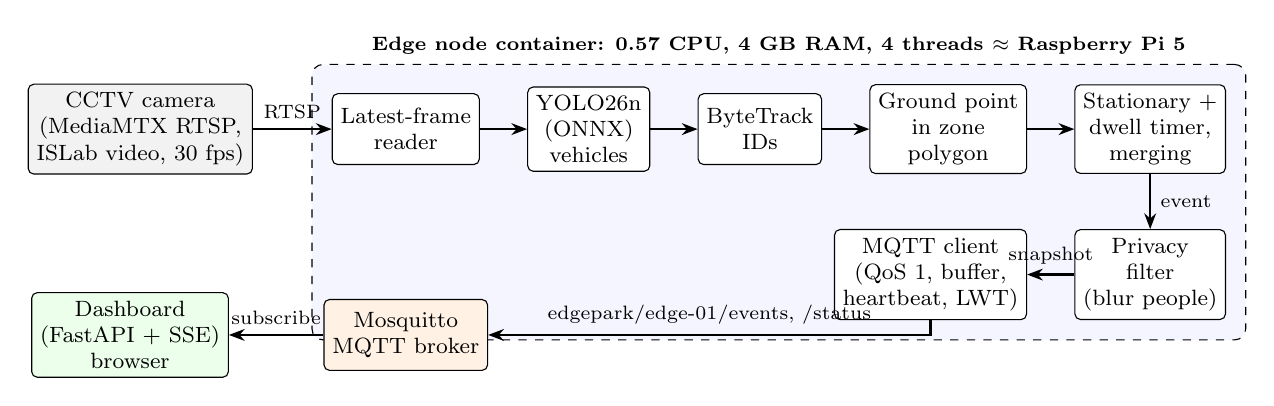
\begin{tikzpicture}[
  node distance=4mm and 6mm,
  box/.style={draw, rounded corners=2pt, align=center, font=\footnotesize, minimum height=9mm, inner sep=3pt, fill=white},
  arr/.style={-{Stealth[length=2mm]}, thick},
  lbl/.style={font=\scriptsize, align=center}]
\node[box, fill=gray!10] (cam) {CCTV camera\\(MediaMTX RTSP,\\ ISLab video, 30 fps)};
\node[box, right=10mm of cam] (grab) {Latest-frame\\reader};
\node[box, right=of grab] (det) {YOLO26n\\(ONNX)\\vehicles};
\node[box, right=of det] (trk) {ByteTrack\\IDs};
\node[box, right=of trk] (zone) {Ground point\\in zone\\polygon};
\node[box, right=of zone] (dwell) {Stationary +\\dwell timer,\\merging};
\node[box, below=7mm of dwell] (priv) {Privacy\\filter\\(blur people)};
\node[box, left=of priv] (pub) {MQTT client\\(QoS 1, buffer,\\heartbeat, LWT)};
\begin{scope}[on background layer]
\node[draw, dashed, rounded corners, fill=blue!4, inner sep=2.5mm, fit=(grab)(det)(trk)(zone)(dwell)(priv)(pub), label={[font=\scriptsize\bfseries]above:{Edge node container: 0.57 CPU, 4 GB RAM, 4 threads $\approx$ Raspberry Pi 5}}] (edge) {};
\end{scope}
\node[box, fill=orange!10, below=17mm of grab] (broker) {Mosquitto\\MQTT broker};
\node[box, fill=green!8, left=12mm of broker] (dash) {Dashboard\\(FastAPI + SSE)\\browser};
\draw[arr] (cam) -- node[lbl, above] {RTSP} (grab);
\draw[arr] (grab) -- (det);
\draw[arr] (det) -- (trk);
\draw[arr] (trk) -- (zone);
\draw[arr] (zone) -- (dwell);
\draw[arr] (dwell) -- node[lbl, right] {event} (priv);
\draw[arr] (priv) -- node[lbl, above] {snapshot} (pub);
\draw[arr] (pub) |- node[lbl, pos=0.75, above] {edgepark/edge-01/events, /status} (broker);
\draw[arr] (broker) -- node[lbl, above] {subscribe} (dash);
\end{tikzpicture}}
\caption{EdgePark architecture. Each block is a Docker container; the dashed box is the CPU- and memory-limited edge node.}
\label{fig:arch}
\end{figure*}

\subsection{Frame Acquisition}
On a live stream the node cannot analyse all 30 frames per second, and processing a backlog would delay every alert. A background thread therefore keeps reading the RTSP stream and stores only the newest frame; the analysis loop always takes that frame, and older frames are dropped. All timing in the pipeline uses the capture time of the frame, so the dwell logic does not depend on how many frames the node manages per second. For offline experiments the same code reads video files at a fixed analysis rate.

\subsection{Vehicle Detection}
The detector is a COCO-pretrained YOLO model~\cite{ultralytics,lin2014coco} used without fine-tuning; the classes car, motorcycle, bus and truck are kept. Three nano models were compared: YOLOv8n, YOLO11n and YOLO26n. Each was exported to ONNX and NCNN in addition to PyTorch. The deployed configuration is YOLO26n in ONNX Runtime at 640~px input (Section~\ref{sec:results}).

\subsection{Tracking}
ByteTrack~\cite{zhang2022bytetrack} links detections across frames. It also uses low-confidence boxes to keep tracks alive, which helps with partly hidden parked vehicles. We use a high threshold of 0.25, a low threshold of 0.1 and a track buffer of about 3 s.

\subsection{Restricted Zones}
Zones are polygons drawn on each camera view, one YAML file per camera. They follow a written policy agreed before any results were seen. Restricted areas are fire lanes and narrow access roads, no-parking curb strips, entrances and driveways, crosswalks, and roundabout edges. Live traffic lanes, marked parking spaces and areas where vehicles are too small to detect reliably are excluded. A vehicle is inside a zone when its ground point, the bottom centre of its box,
\begin{equation}
g = \left(\tfrac{x_1 + x_2}{2},\; y_2\right),
\label{eq:ground}
\end{equation}
lies in the polygon. The ground point marks where the vehicle touches the road, while the box centre used by the baseline~\cite{daluz2026} can fall inside a zone when the vehicle stands next to it.

\subsection{Dwell-Time Logic}
For each tracked vehicle the node keeps the ground points of the last $\tau = 2$ s. The vehicle is stationary when
\begin{equation}
\max_{k \in W_t} \lVert g_t - g_k \rVert \leq \rho\, h_t, \qquad \rho = 0.15,
\label{eq:still}
\end{equation}
where $W_t$ is the window and $h_t$ the box height, so the tolerance scales with distance from the camera. The time $t_s$ at which the vehicle became stationary starts its dwell timer, and a violation is raised when
\begin{equation}
d_t = t - t_s \geq T .
\label{eq:dwell}
\end{equation}
Only real movement resets the timer, so a vehicle that creeps forward in a queue never accumulates time. Algorithm~\ref{alg:dwell} lists the update for one frame. Three measures prevent repeated alerts. First, each vehicle raises at most one violation event, which stays open until a \emph{cleared} event. Second, if the tracker loses a vehicle and gives it a new identity, the new track inherits the old state when their boxes overlap by IoU $\geq 0.5$ within a grace period of 5 s. Third, a second box on the same vehicle in the same frame (IoU $\geq 0.7$, or ground points closer than 0.2 box heights) is merged into it.

\begin{algorithm}[!t]
\caption{Dwell-time update for one analysed frame}
\label{alg:dwell}
\footnotesize
\begin{algorithmic}[1]
\Require frame time $t$, tracked vehicle boxes $B$, zones $Z$, states $S$
\For{each box $b \in B$ with ground point $g$ in a zone $z$}
  \If{$b$ duplicates a vehicle already handled at $t$} \textbf{continue} \EndIf
  \State $s \gets S[\mathrm{id}(b)]$, or a recently lost state with IoU $\geq 0.5$, or a new state
  \State append $(t, g, h)$ to the history of $s$; drop samples older than $\tau$
  \If{$s$ moved more than $\rho h$ \textbf{and} no alert yet} $t_s \gets$ none
  \ElsIf{$s$ still for the whole window \textbf{and} $t_s =$ none} $t_s \gets$ start of window
  \EndIf
  \If{no alert yet \textbf{and} $t - t_s \geq T$} emit \textsc{violation}$(s)$ \EndIf
\EndFor
\For{each state $s$ not seen for more than the grace period}
  \If{$s$ had an alert} emit \textsc{cleared}$(s)$ \EndIf
  \State remove $s$
\EndFor
\end{algorithmic}
\end{algorithm}

\subsection{Alerting over MQTT}
Events are published to \texttt{edgepark/<node>/events} with QoS~1, so each is delivered at least once. A violation message carries the event and track identifiers, zone, vehicle class, stop time, dwell time, box, the capture time of the triggering frame and a JPEG snapshot of at most 480 px width. Every 5 s the node publishes a retained heartbeat on \texttt{edgepark/<node>/status} with its frame rate, inference time and number of vehicles in view; a last-will message marks the node offline if its connection drops. The MQTT client runs in its own thread and queues up to 1,000 messages while the broker is unreachable, so a network outage never stalls detection. Every event is also logged locally.

\subsection{Privacy}
Before a snapshot leaves the node, people in it are detected with the same COCO model and blurred. For material shared publicly (this report, slides, demo videos) vehicles can also be pixelated so that number plates cannot be read.

\subsection{Dashboard}
The dashboard subscribes to all nodes and keeps the open violations, recent history and node status in memory. Browsers receive changes immediately through Server-Sent Events and show each violation with its snapshot, zone, dwell time and capture-to-dashboard latency (Fig.~\ref{fig:dash}). Each event carries a run identifier, so violations left open by a node that restarts are removed instead of staying on screen.

\subsection{Raspberry Pi~5 Simulation and Calibration}
No Raspberry Pi was available, so the edge node runs in a container with a CPU quota. To choose the quota we measured the inference time of YOLO26n in PyTorch (FP32, 640~px, batch 1, coco128, the protocol of the Ultralytics Raspberry Pi guide~\cite{ultralyticspi}) at several CPU limits. We then interpolated the limit $c^*$ that matches the published Pi~5 time $L^* = 299$ ms on a log--log scale between the two measured limits $c_1, c_2$ that bracket it:
\begin{equation}
\ln c^* = \ln c_1 + \frac{\ln L^* - \ln L_1}{\ln L_2 - \ln L_1}\left(\ln c_2 - \ln c_1\right).
\label{eq:cal}
\end{equation}
The calibration error of a runtime $f$ is $e_f = (L_f^{\text{sim}} - L_f^{\text{Pi5}}) / L_f^{\text{Pi5}}$.

%=====================================================================
\section{Experimental Setup}
%=====================================================================
\subsection{Datasets}
Table~\ref{tab:data} lists the data. The ISLab parking-violation dataset~\cite{islabpvd} contains 16 videos from fixed CCTV cameras in six scenes: a roundabout, a curbed road, a narrow alley used as a fire lane, a campus road with a parking-lot entrance, a parking-lot driveway and a road at night in infrared. UA-DETRAC~\cite{wen2020detrac} provides roadside frames with a box for every vehicle; we took every tenth annotated frame of two test sequences per weather type. Coco128 is used only for the speed protocol, so that our times are comparable with the published Pi~5 figures.

\begin{table}[!t]
\caption{Datasets and their roles}
\label{tab:data}
\centering
\footnotesize
\begin{tabularx}{\columnwidth}{@{}p{1.5cm}p{1.5cm}X@{}}
\toprule
Dataset & Used for & Content \\
\midrule
ISLab PVD \cite{islabpvd} & Alert quality & 16 videos, 2,991 s, $\sim$640$\times$480, 20/30 fps; 20 labelled stop events; dev 5 videos, test 11 \\
UA-DETRAC \cite{wen2020detrac} & Detection accuracy & 842 frames from 8 sequences, 5,714 vehicle boxes (sunny, cloudy, rainy, night) \\
coco128 \cite{lin2014coco} & Speed & 128 images, published Pi~5 protocol \\
\bottomrule
\end{tabularx}
\end{table}

\subsection{Ground Truth and Data Split}
The ISLab videos have no event labels, so we labelled every stop of a vehicle inside a zone with its stop and leave times. Labels were read from frames sampled every 5 s, and every second around events that last close to 60 s. Events whose zone membership could not be decided were marked ambiguous and count neither for nor against a method. To avoid tuning on test data, videos 01, 04, 07, 08 and 15 form the development set, used for building and tuning. The remaining 11 videos form the test set and were used only for the final numbers. Zones were frozen before the test results were computed.

\subsection{Metrics}
Detection is scored with precision, recall and mAP over IoU thresholds 0.50:0.05:0.95, treating all vehicle types as one class and ignoring detections in the DETRAC ignore regions. An alert is a true positive when it falls inside a labelled event of the same zone and vehicle type, with a tolerance of 5 s. Further alerts for an already matched event are duplicates, and alerts that match no event are false alarms:
\begin{equation}
P = \frac{TP}{TP + FP + D}, \qquad R = \frac{TP}{N_v}, \qquad F_1 = \frac{2PR}{P + R},
\label{eq:pr}
\end{equation}
where $D$ is the number of duplicates and $N_v$ the number of violations, that is, events at least $T$ seconds long. Speed is the median inference time of three runs.

\subsection{Baseline and Variants}
The baseline replicates the rule of da Luz et al.~\cite{daluz2026}: in every analysed frame each vehicle whose box centre lies in a zone produces an alert. To measure each component we also run nested variants: (A) the ground point, frame-wise; (B) tracking, alert on zone entry; (C) a dwell timer per zone without identities; (D) tracking and dwell without duplicate merging; and (E) the full system. Detection and tracking were run once per video at 3 frames per second, the rate of the calibrated node. All variants replay the same tracks, so their differences come only from the alert logic.

\subsection{Implementation Settings}
Table~\ref{tab:settings} lists the software and parameters.

\begin{table}[!t]
\caption{Implementation settings}
\label{tab:settings}
\centering
\footnotesize
\begin{tabularx}{\columnwidth}{@{}p{2.3cm}X@{}}
\toprule
Item & Value \\
\midrule
Software & Python 3.11, Ultralytics 8.4, PyTorch 2.15 (CPU), ONNX Runtime 1.32, OpenCV, paho-mqtt 2, FastAPI, Docker 29 \\
Host & Intel Core i5-8250U laptop, WSL2 with 4 vCPUs and 8 GB, on mains power \\
Edge container & 0.57 CPU, 4 GB RAM, 4 inference threads \\
Detector & 640 px; detection confidence 0.35 \\
ByteTrack & high/low thresholds 0.25/0.1, buffer $\approx$3 s \\
Dwell rule & $\rho = 0.15$, $\tau = 2$ s, grace 5 s, $T \in \{10, 30, 60\}$ s \\
MQTT & QoS 1 events, retained heartbeat every 5 s, last will \\
\bottomrule
\end{tabularx}
\end{table}

%=====================================================================
\section{Results and Discussion}
\label{sec:results}
%=====================================================================
\subsection{Detection Accuracy}
Table~\ref{tab:detrac} gives the detection results on UA-DETRAC. YOLO26n is the most accurate model on every metric; it gains 0.027 mAP@0.5:0.95 and 3.4 points of recall over YOLOv8n. The ranking YOLOv8n $<$ YOLO11n $<$ YOLO26n holds in all four weather conditions (Fig.~\ref{fig:weather}). Cloudy frames are the hardest for all three models. The night sequences score highest because the DETRAC night scenes are well lit by street lamps.

\begin{table}[!t]
\caption{Vehicle detection on UA-DETRAC (842 frames)}
\label{tab:detrac}
\centering
\footnotesize
\begin{tabular}{@{}lccccc@{}}
\toprule
Model & P & R & F1 & mAP@0.5 & mAP@0.5:0.95 \\
\midrule
YOLOv8n & 0.883 & 0.753 & 0.813 & 0.815 & 0.555 \\
YOLO11n & 0.879 & 0.783 & 0.828 & 0.836 & 0.575 \\
YOLO26n & \textbf{0.886} & \textbf{0.787} & \textbf{0.833} & \textbf{0.841} & \textbf{0.582} \\
\bottomrule
\end{tabular}
\end{table}

\begin{figure}[!t]
\centering
\img{fig_detrac_map_by_weather.pdf}{\columnwidth}
\caption{mAP@0.5:0.95 per weather condition on UA-DETRAC.}
\label{fig:weather}
\end{figure}

\subsection{Speed on the Simulated Raspberry Pi~5}
Fig.~\ref{fig:cal} shows the calibration sweep. Interpolation gives a limit of 0.57 CPU, at which YOLO26n in PyTorch takes 302 ms per image (runs of 297, 302 and 304 ms) against the published 299 ms. Table~\ref{tab:speed} lists all models and formats at this limit. ONNX is the fastest format for every model: it cuts YOLO26n from 286 to 187 ms (35\%) and YOLO11n from 304 to 195 ms, while the coco128 mAP changes by at most 0.010. NCNN beats PyTorch for YOLOv8n and YOLO11n but is slower for YOLO26n.

\begin{figure}[!t]
\centering
\img{fig_calibration_curve.pdf}{\columnwidth}
\caption{Inference time of YOLO26n (PyTorch) versus container CPU limit; the dashed line is the published Raspberry Pi~5 time.}
\label{fig:cal}
\end{figure}

\begin{table}[!t]
\caption{Inference time (ms/image) on the simulated Pi~5}
\label{tab:speed}
\centering
\footnotesize
\begin{tabular}{@{}lcccc@{}}
\toprule
Model & PyTorch & ONNX & NCNN & mAP coco128 (PT/ONNX) \\
\midrule
YOLOv8n & 315.3 & 224.6 & 259.6 & 0.447 / 0.452 \\
YOLO11n & 303.9 & 194.6 & 267.9 & 0.508 / 0.505 \\
YOLO26n & 285.8 & \textbf{187.2} & 310.7 & 0.487 / 0.477 \\
\midrule
Real Pi 5, 26n \cite{ultralyticspi} & 299.1 & 126.0 & 67.0 & -- \\
Simulation error & $-$4.4\% & +48.6\% & +363.5\% & -- \\
\bottomrule
\end{tabular}
\end{table}

The last rows of Table~\ref{tab:speed} and Fig.~\ref{fig:sim} test the simulation itself. The calibrated container matches the real board for PyTorch, the format it was calibrated on, but it is 49\% too slow for ONNX and almost five times too slow for NCNN. NCNN is optimised for ARM NEON instructions, which the x86 host does not have. A CPU quota therefore models the \emph{amount} of compute, not the instruction set. Absolute times for other runtimes, and the ranking between ONNX and NCNN, do not carry over from an x86 simulation to an ARM board; on a real Pi~5 NCNN would be the fastest format.

\begin{figure}[!t]
\centering
\img{fig_sim_vs_real_pi5.pdf}{\columnwidth}
\caption{Simulated versus published Raspberry Pi~5 inference time of YOLO26n per runtime.}
\label{fig:sim}
\end{figure}

For deployment (RQ3) we chose YOLO26n in ONNX, the most accurate model in the fastest format that our simulation can measure. In the complete pipeline at Pi~5 speed (decoding, inference, tracking, zone and dwell logic) the node processes about 4 frames per second. Fig.~\ref{fig:frames} shows its output on the fire-lane scene.

\begin{figure}[!t]
\centering
\img{frames_07.jpg}{\columnwidth}
\caption{Pipeline output on ISLab video 07 (fire lane, $T$ = 60 s). Left: the SUV drives in and is tracked but not reported (white), while the parked motorbike's dwell timer runs (yellow). Middle: the motorbike reaches 60 s and becomes a violation (red); the SUV now stands still and its timer runs. Right: the SUV is reported too. Vehicles are pixelated for privacy.}
\label{fig:frames}
\end{figure}

\subsection{Alert Quality}
Table~\ref{tab:alerts} compares the baseline with EdgePark on the 11 test videos. The frame-wise baseline finds every violation, but it produces 1,776 alerts for 9 violations. 159 of them are false alarms on vehicles that only pass or stop briefly, and 1,608 are repeats for the same vehicle, so its precision is 0.005. With $T = 30$ s EdgePark raises 9 alerts for 10 violations, all correct (precision 1.000, recall 0.900, F1 0.947). With $T = 60$ s it raises 5 alerts, again all correct, but misses 4 of the 9 longer stops. Alerts arrive on average 1.0--2.2 s after the vehicle reaches the threshold, the time the node needs to confirm that the vehicle has been still.

\begin{table}[!t]
\caption{Alert quality on the 11 test videos}
\label{tab:alerts}
\centering
\footnotesize
\begin{tabular}{@{}llrrrrrr@{}}
\toprule
$T$ & Method & Alerts & TP & FP & Dup. & P & R \\
\midrule
30 s & Frame-wise ROI \cite{daluz2026} & 1,776 & 9 & 159 & 1,608 & 0.005 & 0.900 \\
30 s & EdgePark & 9 & 9 & 0 & 0 & \textbf{1.000} & 0.900 \\
60 s & Frame-wise ROI \cite{daluz2026} & 1,776 & 9 & 159 & 1,608 & 0.005 & 1.000 \\
60 s & EdgePark & 5 & 5 & 0 & 0 & \textbf{1.000} & 0.556 \\
\bottomrule
\end{tabular}
\end{table}

\subsection{Ablation}
Table~\ref{tab:ablation} and Fig.~\ref{fig:variants} add the components one at a time. Using the ground point alone (A) does not help, because a frame-wise rule still repeats itself every frame. Tracking with an alert on zone entry (B) removes most repeats (2,700 to 35 alerts), but passing vehicles still trigger alerts. The dwell timer brings the largest gain in precision (C). Tracking matters for recall: a zone-level timer without identities cannot separate two vehicles in the same zone (C 0.700 vs.\ D 0.900 recall at 30 s). Duplicate merging removes the last repeated alert without losing a violation (D 10 alerts, E 9).

\begin{table}[!t]
\caption{Ablation on the test videos}
\label{tab:ablation}
\centering
\footnotesize
\begin{tabular}{@{}lrrrrrr@{}}
\toprule
Variant & \multicolumn{3}{c}{$T = 30$ s} & \multicolumn{3}{c}{$T = 60$ s} \\
 & Alerts & P & R & Alerts & P & R \\
\midrule
Baseline, box centre & 1,776 & 0.005 & 0.900 & 1,776 & 0.005 & 1.000 \\
A ground point & 2,700 & 0.003 & 0.900 & 2,700 & 0.003 & 0.889 \\
B + tracking & 35 & 0.229 & 0.800 & 35 & 0.200 & 0.778 \\
C dwell, no IDs & 8 & 0.875 & 0.700 & 5 & 1.000 & 0.556 \\
D tracking + dwell & 10 & 0.900 & 0.900 & 5 & 1.000 & 0.556 \\
E full (EdgePark) & 9 & \textbf{1.000} & 0.900 & 5 & \textbf{1.000} & 0.556 \\
\bottomrule
\end{tabular}
\end{table}

\begin{figure}[!t]
\centering
\img{fig_alert_variants.pdf}{\columnwidth}
\caption{Precision and recall of the variants on the test videos at $T$ = 60 s.}
\label{fig:variants}
\end{figure}

\subsection{Threshold and Parameter Sensitivity}
The threshold $T$ sets the trade-off between early and certain alerts (Fig.~\ref{fig:thresh}). On the test videos the full system reaches P = R = 0.818 at $T = 10$ s, P = 1.000 and R = 0.900 at 30 s, and P = 1.000 and R = 0.556 at 60 s. Short thresholds report vehicles that stop briefly; long thresholds lose vehicles whose timer is interrupted, for example by an occlusion. The occlusion grace period was tuned on the development videos only. Every value from 5 to 20 s gave the same development F1 of 0.941, so we kept 5 s. The development results (P 0.889, R 1.000 at 60 s) are not worse than the test results, so the parameters were not over-fitted to the development set.

\begin{figure}[!t]
\centering
\img{fig_threshold_sensitivity.pdf}{\columnwidth}
\caption{Effect of the dwell threshold $T$ on the full system (test videos).}
\label{fig:thresh}
\end{figure}

\subsection{Live System Performance}
Running the complete Docker deployment (Fig.~\ref{fig:arch}) on the fire-lane video, the edge node raised one violation for the parked motorbike and one for the SUV, and a \emph{cleared} event when the SUV left. The node processed 4--4.7 frames per second (about 205--218 ms per frame including tracking). Measured at the dashboard, alerts arrived 0.3--0.9 s after their frame was captured. Almost all of this time is inference: the MQTT hop from the node through the broker to the dashboard took 2--60 ms. The node used about 170 MB of its 4 GB memory limit. The host power mode matters: on battery in Windows' balanced mode, the same CPU limit gave unstable inference times up to three times slower, and the node fell to about 1.9 frames per second. All speed results in this report were therefore measured on mains power in best-performance mode.

\begin{figure}[!t]
\centering
\img{dashboard.jpg}{\columnwidth}
\caption{Dashboard during the live run: two open violations with their privacy-filtered snapshots, mean capture-to-dashboard latency and node status.}
\label{fig:dash}
\end{figure}

\subsection{Failure Analysis}
We traced the four violations missed at $T = 60$ s. In video 13 the vehicle stood about 10 pixels outside the edge of the entrance zone. In video 16 a vehicle parked diagonally close to the night camera, and its ground point fell 33 pixels into the traffic lane. The baseline counted both because their box centres lay inside the zones. The ground point is reliable for side views but not for large vehicles seen at a steep angle. In video 10 a person stood next to a parked motorbike; its box shifted and the timer restarted after 50 s. In video 02 the vehicle was only 13--14 pixels high and was first detected about 20 s after it stopped. We did not change the test zones after seeing these errors, since that would bias the evaluation.

%=====================================================================
\section{Limitations}
%=====================================================================
The edge device is simulated, and its calibration is valid only for PyTorch, so ONNX and NCNN speeds on a real Pi~5 will differ (Table~\ref{tab:speed}). The ground-truth labels were produced in a single pass by an AI assistant inspecting sampled frames, at the team's request (a provenance note is kept in the label file), and stop and leave times are known to within 1--7.5 s. The test set holds 9 violations at $T = 60$ s, so one missed event changes recall by 0.11. Detection ran at 3 frames per second, and faster hardware could follow occlusions better. The zones come from a written policy because the real parking rules of the filmed sites are unknown.

%=====================================================================
\section{Conclusion and Future Work}
%=====================================================================
EdgePark detects restricted-zone parking violations on a Raspberry Pi~5 class edge node and reports them over MQTT to a live dashboard. Tracking and a stationary-aware dwell timer turn 1,776 frame-wise alerts into 9 correct ones at a 30 s threshold. YOLO26n in ONNX was the most accurate and fastest of the tested configurations at 187 ms per image. A calibrated CPU-limited container is a good stand-in for the board only for the runtime it was calibrated on. Future work: run the node on a real Raspberry Pi~5 with NCNN, make the ground point depend on the camera angle, keep the dwell timer running through short occlusions by people, add a second annotator and more violation videos, and support several cameras per node.

\section*{Code Availability}
Code, zone definitions, ground truth, result files and the step-by-step demo are available at \url{https://github.com/Ab-21651/Restricted-Zone-Parking-Violation-Detection}. Every number in this report can be regenerated with the scripts listed in the repository README.

\section*{Acknowledgment}
An AI coding assistant (Claude, Anthropic) was used during this project. Its contributions are listed in the ``AI assistance'' section of the repository README.

\bibliographystyle{IEEEtran}
\bibliography{references}

\end{document}
